% !TEX root = sum1.tex
\section{Problem Description}
In this section, we give the description of the seat planning problem with social distance. Then we consider the dynamic seat assignment problem with social distance.

% First, we will introduce some preliminary knowledge about our problem as follows.

\subsection{Dynamic Seat Assignment Problem with Social Distance}\label{dynamic_demand}

We mainly focus on the dynamic seat assignment problem, which is suitable for commercial use. In this situation, customers come dynamically and the seating plan needs to be made without knowing the number and composition of future customers. It becomes a sequential stochastic optimization problem where conventional methods fall into the curse of dimensionality due to many seating plan combinations. 

For example, the dynamic programming for this problem is

% We use a vector to record the state of each row, in every period the group can decide which row to sit.

$$V_{t}(\mathbf{S}_{t}) = \sum_{i \in N} p_i \max\{ {[V_{t-1}(\mathbf{S}_{t-1}^{1})+ s_i]}, {V_{t-1}(\mathbf{S}_{t}^{0})}\}$$

where $\mathbf{S}_{t} = (S_1^{t}, S_2^{t}, \ldots, S_{N}^{t})$ represents the state of each row, $\mathbf{S}_{t-1}^{1} = (S_1^{t-1}, S_2^{t-1}, \ldots, S_{N}^{t-1})$ is the state when accepting the group. If placing the group type $i$ in row $j$, then $S_{j}^{t-1} = S_{j}-s_{i}-1$, $S_{k}^{t-1} = S_{j}^{t}, k \neq j$. $\mathbf{S}_{t-1}^{0} = \mathbf{S}_{t}$ is the state when rejecting the group. Initially, we have $\mathbf{S}_{T} = (S_1, S_2, \ldots, S_{N})$.

As we can see, this dynamic programming is difficult to calculate with large dimension. To avoid this complexity, we develop an approach that aims directly at the final seating plans, then make the policy to assign groups. We discuss two dynamic situations in the following section to further know how to make decisions when the group arrives dynamically.


% As stated above, we can obtain such a seating plan from stochastic programming. However, it only gives the initial seat assignment without handling the dynamic situation. 


\subsection{Seat Planning Problem with Social Distance}
% In this section we present the model that generates seat assignment under deterministic demands.

Consider a set of groups, each consisting of no more than $m$ people, to be assigned to a set of seats. These groups are denoted by a demand vector, $\mathbf{d} = (d_1, \ldots, d_m)$. Each element, $d_i, 1 \leq i \leq m$, indicates the number of group type $i$ containing $i$ people. For illustration, we consider the layout as $N$ rows, each row with $S_{j}$ seats, $j = 1, \ldots, N$. 

% Let the $i-$th group type contain $i$ people. 
% $(d_1, d_2, d_3, d_4) = (3,5,7,6)$

% But our model and formulation allow for a more general layout of the seats. 
According to the epidemic prevention requirements, the customers from the same group can sit together, while different groups should sit with social distancing. 
Suppose that each group has to leave one seat to maintain social distancing from the adjacent groups and different rows have no effect on each other, i.e., a person from one group can sit directly behind a person from another group.

% Considering the actual situation, social distancing is one seat in our paper 
To simplify the social distancing in the seat assignment, we add one to the original size of each group as the new size of the group and one dummy seat to each row. Take $s_{i} = i + 1$, $L_{j} = S_{j} +1$, $s_{i}$ is the new size of group type $i$ and $L_{j}$ is the length of row $j$.

Then we can illustrate the seat planning for one row below. 

\begin{figure}[ht]
    \centering
    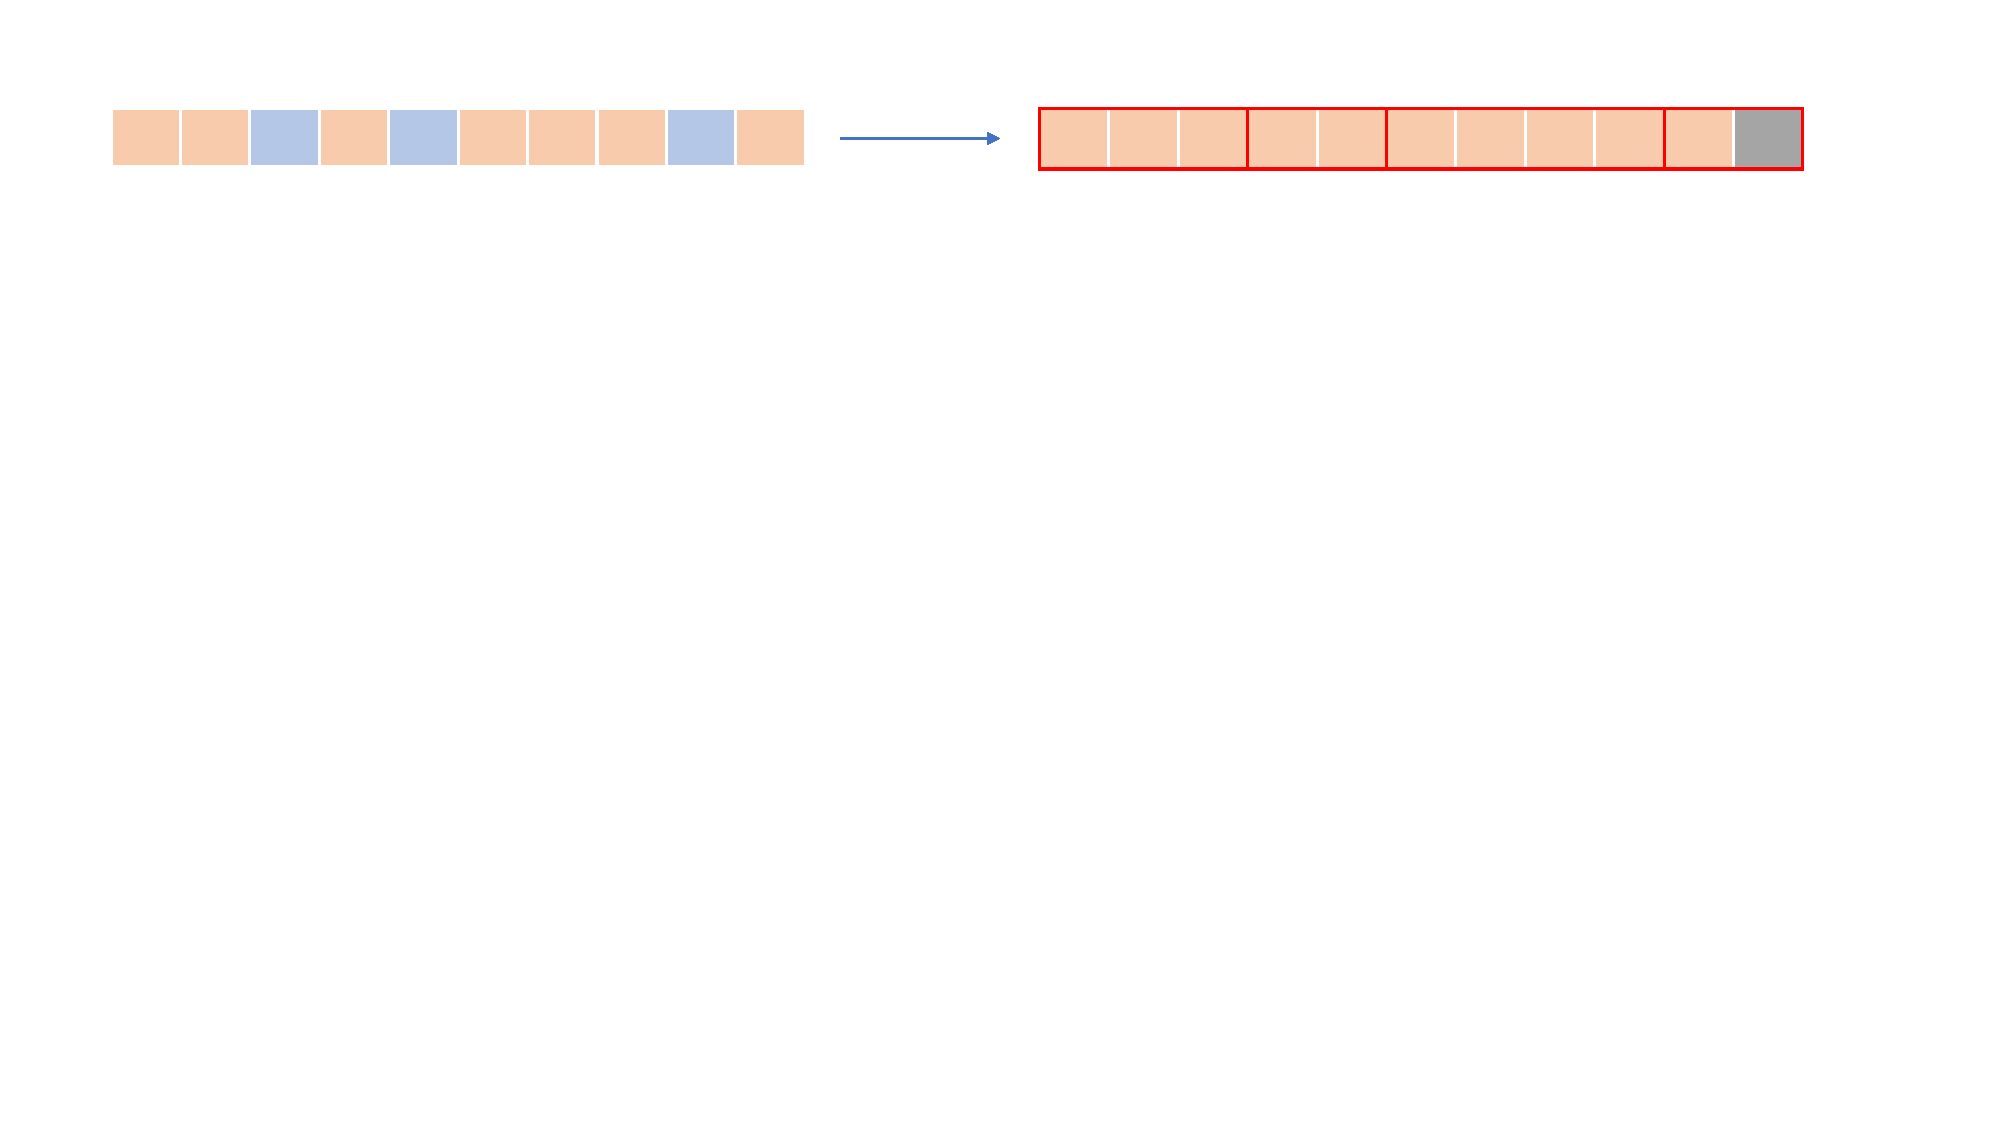
\includegraphics[width = 0.8\textwidth]{./Figures/dummy_seat.pdf}
    \caption{Problem Conversion}
\end{figure}

On the left side, the blue squares stand for the empty seats as the social distancing. The orange squares represent the seats sat by the groups. 
On the right side, one dummy seat is added at the end of the row. The orange squares surrounded by the red line are the seats taken by groups. Here, this row is placed two group of 1, one group of 2 and one group of 3.

In this way, the social distancing can be integrated by solving this seat planning problem.

% The number of all seats in each row is called the length of the row.

% when the capacity allows accepting the groups from large to small as many as possible will give an optimal solution.


% Why is it easy to solve this IP?

% If the ratio is the same for the groups, IP will use more branches to obtain an optimal solution.

% $[24,28,8,9]$ 10 rows.
% Total loss: 60; loss of the largest pattern: 5.


% Specifically, we define the concept of target seating plans deemed satisfactory. In making the dynamic seating plan, we will try to maintain the possibility of achieving one of the target seating plans as much as possible.